% UTF-8

% single-chapter commands
\documentclass[../main/thesis.tex]{subfiles}
\onlyinsubfile{\setcounter{chapter}{5}}  % single-chapter command
\begin{document}


\chapter{Ergebnisdiskussion}
% Beschreibung, was tatsächlich die Software ausspuckt, wo's hakt und wo ich noch gebastelt habe
% alles NUR im "Anwendungskontext", d.h. in Bezug auf die Ausgabe-Geodaten, nicht die Softwarequalität (das war in 5.4!)
% Schritt für Schritt Probleme sammeln und katalogisieren

Die in Kap. 4 und 5 entwickelte Software ist das Ergebnis dieser Arbeit. Hier diskutiert werden soll die Arbeitsweise dieser Software und die Qualität der von ihr ausgegebenen Geodaten in Bezug auf die Aufgabenstellung.

% möglichst auch Untersuchung der Anwendung des Algorithmus auf Straßen in unterschiedlichen Regionen der Welt



\section{Anwendung in einfachen Situationen}

Bei Anwendung der mit dieser Arbeit entwickelten Software auf Geodaten aus der \osm-Datenbank zeigt sich, dass die implementierten Algorithmen grundsätzlich funktionieren.

\onefigure{p}{
	\twofigures{H}{
		\begin{overpic}[width=\ScaleIfNeeded]{../chapter6/result-trivial-in}
			\put(122,84){\figuremark{1}}
			\put(46,46){\figuremark{2}}
		\end{overpic}
	}{
		\begin{overpic}[width=\ScaleIfNeeded]{../chapter6/result-trivial-out}
			\put(122,84){\figuremark{1}}
			\put(46,46){\figuremark{2}}
		\end{overpic}
	}
	% trivial = testbed-nrw/koeln-classfied-nolinks.shp
	% 1:30000 Google Mercator, bbox 778765 6607045 780865 6608245, 0.2mm stroke
	\caption{Ergebnis der Software im einfachen Fall (links Eingangsdaten, rechts Generalisierungsergebnis; Autobahn L~124 bei Köln-Gremberg)}
	\label{fig:result-trivial}
}

In Abbildung~\ref{fig:result-trivial} sind links \osm-Linienzüge in der einfachen Situation einer Autobahn ohne Anschlussstellen nebst innerstädtischen Sammelstraßen zu sehen.
Durch Anwendung der Software ergibt sich das rechts dargestellte automatisiert zusammengefasste Ergebnis.
Anstelle der beiden Richtungsfahrbahnen der Autobahn gibt es nun nur noch eine gemeinsame Mittellinie.
Die Nähe zu nachgeordneten Straßen und deren planfreie Kreuzung mit der Autobahn (bei Markierung~\textfiguremark{1}) stört die Generalisierung nicht.
Auch eine Strecke paralleler Fahrbahnen im nachgeordneten Netz wurde trotz eines scharfen Knicks erfolgreich als parallel erkannt und zusammengefasst (Markierung~\textfiguremark{2}).

Abbildung~\ref{fig:result-trivial-styled} zeigt beispielhaft, wie sich dieses Generalisierungsergebnis sinnvoll visualisieren ließe.
Die Software kennzeichnet die zusammengefassten Linienzüge als generalisiert.
Zusätzlich gibt die Software einzelne \term{tags} der \osm-Quelldaten mit aus.
Anhand dieser Attribute können leicht Regeln mit jeweils passenden Liniearsignaturen definiert werden.

\onefigure{p}{
	\twofigures{H}{
		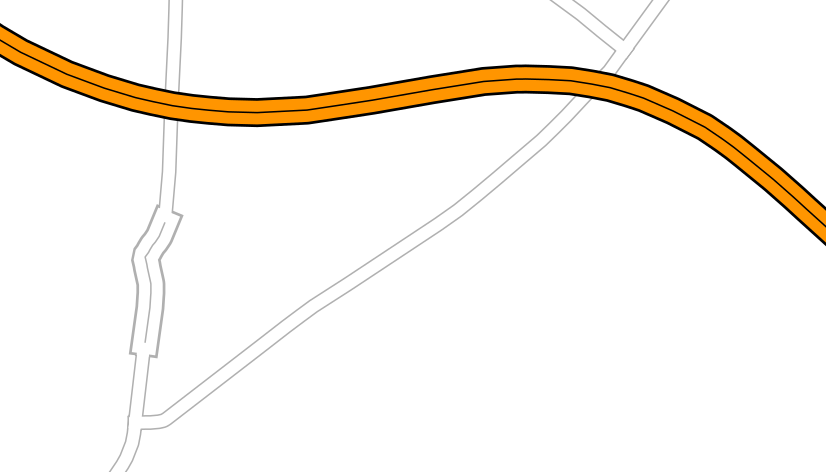
\includegraphics[width=\ScaleIfNeeded]{../chapter6/result-trivial-styled}
	}{
		\includegraphics[width=\ScaleIfNeeded]{../chapter6/result-trivial-rules}
	}
	\caption{Visualisierung des Generalisierungsergebnisses (links Kartendarstellung, rechts Screenshot der Zeichenregeln in QGIS)}
	\label{fig:result-trivial-styled}
}

Bei näherer Betrachtung
% der Autobahn (\textfiguremark{1} in Abbildung~\ref{fig:result-trivial})
ist die beabsichtigte Arbeitsweise der implementierten Algorithmen im einfachen Fall gut zu erkennen (Abbildung~\ref{fig:result-trivial-detail-L124}):
Linienzüge werden durch \textproc{Splitten} derart unterteilt, dass möglichst jeweils zwei Punkte auf Parallelen einander gegenüber liegen (gut zu sehen bei Markierung~\textfiguremark{1}).
Die dabei entstehenden einander gegenüberliegenden Fragmente sind durch ihre Ähnlichkeit offensichtlich einfach auf Parallelität zu prüfen.
Selbst dann, wenn (wie bei \textfiguremark{2}) beim \textproc{Splitten} keine optimalen Paare entstehen, gelingt das \textproc{NodesZuordnen}, solange wenigstens jeweils ein \emph{Teil} der miteinander verglichenen Segmente zueinander parallel ist (\textfiguremark{3}).
Von diesen Zuordnungen der einander gegenüberliegenden \osm-\term{nodes} lässt sich durch Verbindung ihrer Mittelpunkte leicht eine Mittellinie als Ergebnis ableiten.
Von der Präsenz anderer, nicht paralleler Linienzüge lassen sich die Algorithmen nicht beeinflussen (\textfiguremark{4}).

% writeNodeMatches
\onefigure{p}{
	\twofigures{H}{
		\begin{overpic}[width=\ScaleIfNeeded]{../chapter6/result-trivial-detail-L124}
			\put(0,76){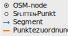
\includegraphics{../chapter6/legend-nodematch}}
			\put(37,50){\figuremark{1}}
			\put(98,56){\figuremark{2}}
			\put(111,56){\figuremark{3}}
			\put(166,52){\figuremark{4}}
		\end{overpic}
	}{
		\begin{overpic}[width=\ScaleIfNeeded]{../chapter6/result-trivial-detail-L124-gen}
			\put(37,50){\figuremark{1}}
			\put(98,56){\figuremark{2}}
			\put(111,56){\figuremark{3}}
			\put(166,52){\figuremark{4}}
		\end{overpic}
	}
	% 1:7500 Google Mercator, bbox 779845 6607935 780370 6608240
	\caption{Detaildarstellung Autobahn mit Punktezuordnungen (links Eingangsdaten, rechts Generalisierungsergebnis; \textfiguremark{1}~in Abbildung~\ref{fig:result-trivial})}
	\label{fig:result-trivial-detail-L124}
}

\begin{itemize}
\item möglichst quantifizieren („bei Eingabedaten von xy km Autobahn gibt es z Problemsituationen“)
\item offen: Nicht-motorway/trunk sind schwieriger, da kleinere Kurvenradien. Funktioniert's hier? Wo nicht?
\item offen: Die \textproc{Distanz} zweier Straßen ist eines der wesentlichen Kriterien für die Erkennung als \textproc{Parallel}. Macht das Probleme, zB innerstädtisch vs. Autobahn?
\end{itemize}



\section{Attribute}

\begin{itemize}
\item (vorläufig) implementiertes Prinzip beschreiben
\item Auswirkungen: Beispiel, wo es nicht klappt?
\item möglichst quantifizieren
\end{itemize}



\section{Verhalten an Straßenkreuzungen}

\subsection{relocateGeneralisedNodes}

\begin{itemize}
\item tlws. gelöstes Problem: an Ende der Ausbaustrecke sowie innerstädtischer Kreuzung nodes von (nicht generalisierter) Querstraße so verschieben, dass es passt
\item offen: löst Problem nicht vollständig: funktioniert nicht (?), wenn Querstraße generalisiert ist?
\item (auch Problem im trivialen Fall, etwa in Heumar oder Kanalstraße/A57: Lücke in Topologie)
% Dass einander kreuzende Autobahnen durch Rampen miteinander verbunden sind, lehrt die Lebenserfahrung; aus dem Generalisierungsergebnis geht es jedoch nicht hervor.
\item möglichst quantifizieren
\end{itemize}

% relocateGeneralisedNodes: "This is necessary because nodes are implemented as immutable by this project." -> Alternative: beide Nodes auf denselben Ort bewegen und dann als letzten Schritt Nodes am selben Ort erkennen und zusammenfassen (dann sollten aber sinnvollerweise auch die Node-IDs mitgeschleppt werden, sonst bringt das wenig, und die haben wir nicht, da wir OSM nicht direkt einlesen, sondern über die Geofabrik-Shapefiles gehen). Wichtig: *nur* wegen relocate() bekommt SourceNode die "edges" als Pointers!

\onefigure{h}{
	\twofigures{H}{
		\begin{overpic}[grid,width=\ScaleIfNeeded]{../chapter6/result-trivial-detail-rolshover}
			\put(0,76){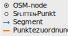
\includegraphics{../chapter6/legend-nodematch}}
%		\put(90,40){\figuremark{1}}
		\put(128,76){\figuremark{1}}
		\end{overpic}
	}{
		\begin{overpic}[width=\ScaleIfNeeded]{../chapter6/result-trivial-detail-rolshover-gen}
		\end{overpic}
	}
	% 1:5000 Google Mercator rotated 55°, bbox 778974 6607426.21 779324 6607629.54
	\caption{Detaildarstellung scharfer Knick mit Punktezuordnungen (links Eingangsdaten, rechts Generalisierungsergebnis; \textfiguremark{2}~in Abbildung~\ref{fig:result-trivial}; Darstellung rotiert)}
	\label{fig:result-trivial-detail-rolshover}
}

Die korrekte Grundfunktionalität ist auch beim scharfen Knick im nachgeordneten Netz
% (\textfiguremark{2} in Abbildung~\ref{fig:result-trivial})
erkennbar (Abbildung~\ref{fig:result-trivial-detail-rolshover}).
Nähere Betrachtung offenbart allerdings einzelne Probleme.
So entstanden in der schwierigen Geometrie direkt beim Knick sich einander kreuzende Punktezuordnungen (Markierung~\textfiguremark{1}).
...

Des Weiteren sei daran erinnert, dass die in Abschnitt~\ref{ch:generalisation-algorithm} gegebene Definition des Algorithmus zum \textproc{Zusammenfassen} keine Behandlung für den Übergang zwischen generalisierten und nicht generalisierten Abschnitten vorsehen.

Anfang und Ende einer Strecke mit zwei Richtungsfahrbahnen vorsehen (Markierung~\textfiguremark{3}).
Um zu vermeiden, dass der generalisierte Linienzug auf der Höhe der letzten Punktezuordnung abrupt und ohne Verbindung zur nicht generaliserten Fortsetzung endet, wurde für diesen Fall in der Software eine Sonderbehandlung vorgesehen, weswegen das Problem im Ergebnis in Abbildungen~\ref{fig:result-trivial} und \ref{fig:result-trivial-styled} nicht existiert.
...

% Ebenso berücksichtigt die Beschreibung weder Kreuzungen noch den Übergang eines einzelnen Linienzugs in zwei parallele Linienzüge.




\subsection{fehlende Kreuzungserkennung}

\begin{itemize}
\item fehlende Kreuzungserkennung
\item umfangreiche Problemdarstellung verschiedener Typen von Kreuzungen
\item möglichst quantifizieren
\end{itemize}



\section{Effizienz}

...



\section{Wiederholtes Ausführen für mehr als zwei Parallele}

...



\section{Anwendung auf andere Spezialfälle}

...



% single-chapter commands
%\onlyinsubfile{\listoffigures}
%\onlyinsubfile{\listoftables}
%\onlyinsubfile{% global bibliography settings

\nocite{*}  % include works in bibliography that aren't cited anywhere in the document (for debugging)

\setbibpreamble{Die Literaturangaben sind alphabetisch nach den Nachnamen der Autoren sortiert. Bei mehreren Autoren wird nach dem ersten Autor sortiert.\par\bigskip\bigskip}

\bibliography{../references-papers,../references-manual}
%\bibliography{../references-manual}
}
\end{document}
